Für das Jahr 2020 wird erwartet, dass 45\% der Weltbevölkerung ein Smartphone nutzt.
% https://www.statista.com/statistics/330695/number-of-smartphone-users-worldwide/
\cite{StatistaSmartphonesWorldwide}
%https://www.statista.com/statistics/262875/development-of-the-world-population/
\cite{StatistaWorldPopulation}
% 3,5 / 7,79 Milliarden = 45%

Unternehmen und Organisationen bedienen diesen mit Markt mit nativen Mobilanwendungen und mobil-optimierten Webseiten.
%Sowohl Unternehmen, die ihre Produkte überwiegend offline vertreiben, als auch die führenden IT-Unternehmen wissen um diesen Trend, denn App-Nutzer sind (potenzielle) Kunden. Auch die Medienbranche verdient mit App-Nutzern Geld, da mit jedem Nutzer ihrer Website oder App die Werbeeinnahmen steigen. 
%Newsportale wie Focus Online, BILD, Welt.de oder Spiegel Online gehören 2019 zu den verbreitetsten mobilen Webseiten \cite{StatistaMobileWebsiteNetReach2019}. Diese  Webseiten sind bereits für Mobilegeräte optimiert. Für Entwickler liegt es nahe, die Webseite in einer Mobilanwendung einzubetten, anstatt alle Features in einer nativen Anwendung neu zu entwickeln. Der Nutzer kann diese Anwendungen über einen App Marktplatz beziehen. Mit Bannern und Links versuchen Unternehmen auf ihre Mobilanwendungen aufmerksam zu machen.
Mit dem Konzept der \ac{pwa} könnte diese zweigleisige Entwicklung bald auf die Webentwicklung reduziert werden: App und Webseite sind hier ein und dieselbe Anwendung. 

% dieser Schritt bald obsolet werden, wenn Nutzer nicht mehr eine plattformabhängige App, sondern vielmehr die Webseite selbst als ``Anwendung'' installieren. Bezieht man die vergleichsweise hohen Entwicklungskosten mobiler Anwendungen in diese Rechnung mit ein, besteht eine große Chance, dass die Erweiterung der bestehenden Webseite zur PWA schneller, wartungärmer und insgesamt günstiger ist.

Die \ac{pwa} verspricht keine eingebettete Webseite, sondern Offline-Funktionalität, Entwicklung mit JavaScript mit Nutzung einer Vielzahl von Bibliotheken und Unabhängigkeit der Plattform und eine flüssige Nutzeroberfläche. Damit löst sie weitverbreitete Probleme von Webanwendungen, welche häufig die Geduld des Nutzers strapazieren. Hier müssen ständig Inhalte (Skripte, Stylesheets, Schriftarten, HTML etc.) über eine langsame mobile Datenverbindung heruntergeladen werden.

Der hohe kombinierte Marktanteil von 80\% des mobilen Browsers Google Chrome (60\% in 2019) und Apple Safari für iOS (20\% in 2019) inspiriert diese Arbeit, die Möglichkeiten der \ac{pwa} im Vergleich zur nativen App ausführlich zu vergleichen. 
%Chrome unter Android unterstützt die PWA bereits vollständig \cite[S. 8]{BeginningPWA} und Apple arbeitet stetig an der Unterstützung der PWA
% (welcher die Installation von PWAs voll unterstützt ) und , welcher die Unterstützung der PWA stetig erweitert,
\cite{StatistaMobileBrowserMarketShare}

% Mobile shopping app user acquisition costs
%https://www.statista.com/statistics/911981/mobile-shopping-apps-user-acquisition-costs-by-type-gender/

% median cost of app dev in regions by $ per hour$
%https://www.statista.com/statistics/628636/worldwide-mobile-app-development-costs-by-region-by-platform/

% median cost of app dev per hour
%https://www.statista.com/statistics/647807/north-america-mobile-app-development-costs/

% market share mobile browsers
%https://www.statista.com/statistics/263517/market-share-held-by-mobile-internet-browsers-worldwide/

% Leading mobile websites ranked by net reach in Germany
%https://www.statista.com/statistics/425372/mobile-websites-by-net-reach-germany/


%\begin{figure}[h]
%        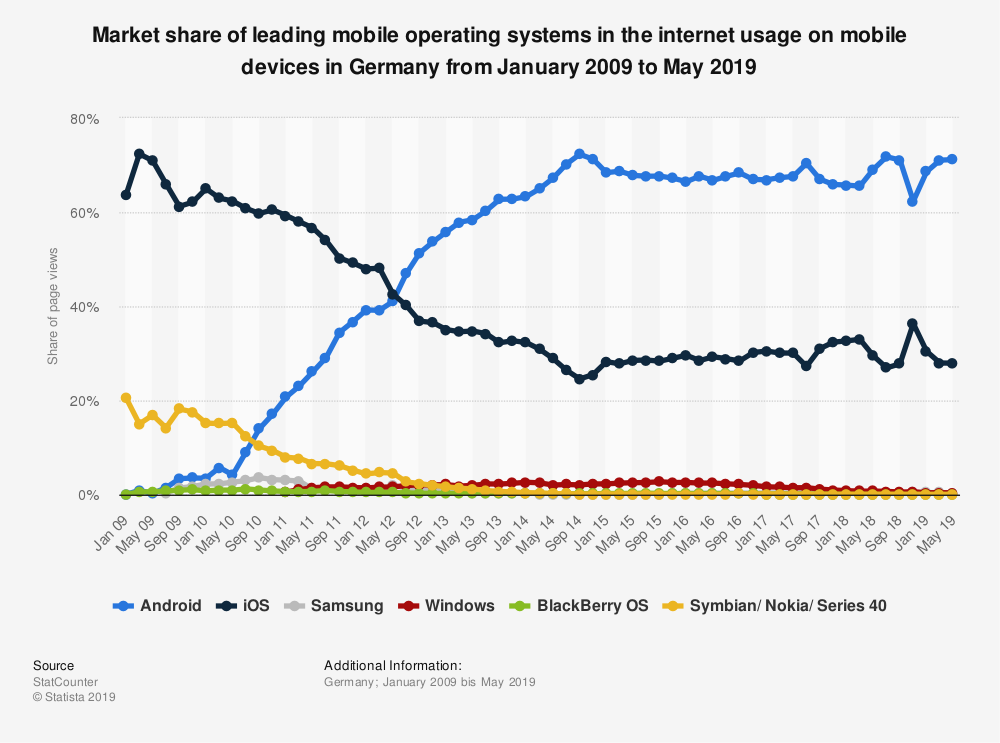
\includegraphics[width=\linewidth]{img/statistic_id461981_market-share-of-operating-systems-in-mobile-internet-usage-in-germany-2009-2019.png}
%        \centering
%        \caption{Market share \cite{StatistaMarketShareSmartphone}}
%        \label{fig:marketshare}
%\end{figure}

